%!TEX root = ../../main.tex
\section{Design og Implementering Software}
Da der skulle laves software blev der taget udgangs punkt i domænemodellen og den gav anledning til følgende opdeling således at
systemet består af følgende software blokke:
\begin{itemize}
\item GUI
\item Database
\item FlexPMS
\item Kar
\item SensorØ
\item Fieldsensor
\item AVSLibrary
\end{itemize}

\subsection{GUI}
GUI er den brugergrænseflade, som brugeren kan tilgå systemet gennem. Som udgangspunkt til at lave GUI'en er der blevet implementeret en webside hvor der er anvendt PHP. Til HTML filerne er der anvendt Bootstrap3, som er beregnet til at gøre webudvikling lettere, da den består af HTML- og CSS- baserede design skabeloner. Ydermere er der anvendt nogle jQuery AJAX metoder, som kan bruges til at udveksle data med en server og opdatere dele af en webside uden at genindlæse hele siden.

\subsection{Database}
Databasen er blevet anvendt til at opbevare indtastede data omkring kar og Sensor Øerne med deres ventil og vandingsstatus, samt aflæste værdier fra de forskellige sensorer, hvor denne database kan tilgås via GUI'en. MySQL er databaseformatet der er valgt, og valget bunder i at denne har alle de kvaliteter systembeskrivelsen og kravspecifikationen foreskriver. Desuden er softwaren til etablering af en sådan server gratis, veldokumenteret og nem at gå til.

\subsection{FlexPMS}
Programmet FlexPMS er designet til at være bindeled mellem brugergrænsefladen og kar/sensorø
styringerne, der til får programmet nogle opgaver der hedder sig at programmet skal op sample
data og gemme dette i databasen, samt holde en log af det opsamlede data. Programmet skal også
facilitere kommunikationen fra brugergrænsefladen til kar/sensorø når der for eksempel bliver bedt
om at starte en vanding i brugergrænsefladen eller det ønskes at styre ventiler. FlexPMS kunne
også udvides således at programmet selv kan bestemme hvornår der skal vandes baseret på de
målinger der er fortaget.

\subsection{Kar}
Kar Controlleren (se \ref{photo:PSoCKar}) er tilkoblet et enkelt Kar, hvor den har en række sensorer og ventiler tilkoblet. Dens funktion er at styre ventilerne baseret på beskeder fra FlexPMS, indsamle data fra dens sensorer tilkoblet karret, indsamle måledata fra Sensor Ø'en og forwarde beskeder videre til SensorØ'en fra FlexPMS. Der er forsøgt at lave automatisk adressering af Sensor Ø'er fra Karret, men da der ingen error detection er på RS485, ligger dette et stykke ude i fremtiden. Sensor Ø'er kan allerede dynamisk oprettes fra FlexPMS.

\begin{figure}[H]
	\centering 
	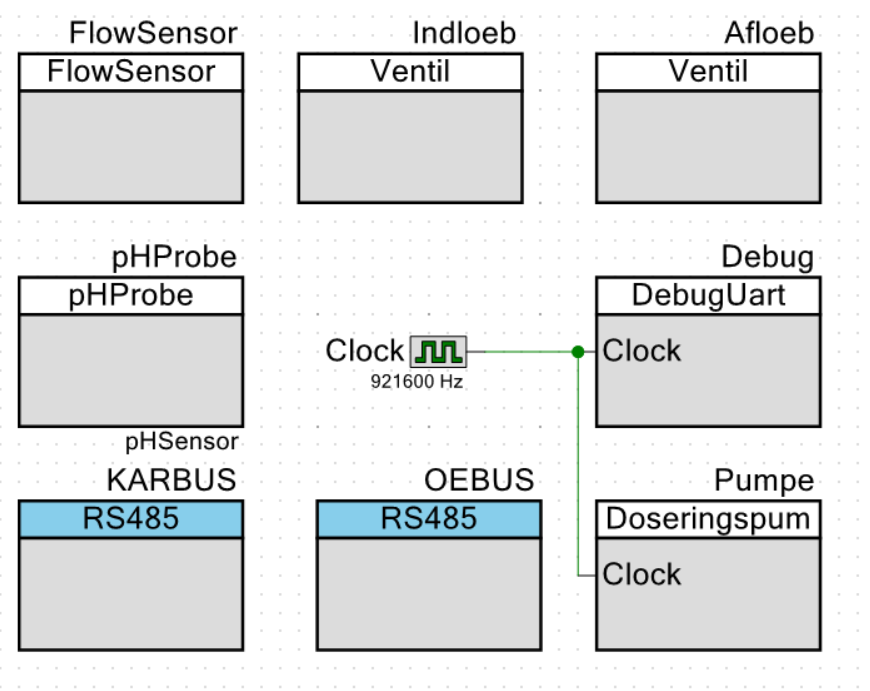
\includegraphics[scale=0.45]{Projektbeskrivelse/DesignOgImplementeringAfSW/Kar/Kar.png}
	\caption{Kar i PSoC creator}
	\label{photo:PSoCKar}
\end{figure}

Det kan ses på figut \ref{photo:PSoCKar} at vi har nydt godt af custom komponenterne fra AVSLibrary, da projektet hurtigt ville have været uoverskuelig og mere errorprone, hvis det hele skulle ha ligget i et enkelt projekt. Nu får man et let overblik over hvad karret reelt indeholder, samt bliver loggikken i projektet lettere at overskue. Den største downside er at man skal være varsom med timings issue som nye komponenter kan introducere.

\subsection{SensorØ}
Sensor Ø'en placeret ude i marken med en række Fieldsensorer og en ventil. Her bliver den brugt til at opsamle data fra dens tilkoblede Fieldsensorer, samt styre ventilen. Mens den afventer beskeder fra Karret, indsamler den data fra Fieldsensoren, derved har den altid de opdaterede tal, når der kommer en forespørgsel fra Karret. Når Sensor Ø'en tændes, scanner den SensorBussen for Fieldsensorer og begynder at polle dem. Der er start implementering på automatisk addresering af Fieldsensorer. 

\subsection{Fieldsensor}
Fieldsensoren er en skabelon til alle typer af Fieldsensorer. Den er bygget til at det er let at udvikle nye sensor typer baseret på skabelonen. Det eneste der skal tilføjes fra udviklerens side er et nyt typeid, samt sørge for at måledata bliver sendt ind via en af skabelonens LoadValue funktioner. Dette gør det lettere at fx skifte kommunikationsinterface, hvis dette skulle være ønsket, da selve sensor udvikleren på intet tidspunkt har skullet rode med den del af koden. Der er lagt start funktioner til automatisk tildeling af I2C adresser, men dette nåede ikke at blive færdigudviklet.

\subsection{AVSLibrary}
AVSLibrary er et bibliotek af custom components \ref{photo:AVSLibrary} til PSoC Creator. Dette er lavet da mange af komponenterne bliver brugt af de forskellige enheder PSoC enheder. Derved sikres det at ændringer bliver rullet ud på tværs af enhederne. En positiv bivirkning er at koden på de andre PSoC enheder bliver lettere at læse, da meget af komponent koden er pakket væk. Der er også implementeret en Debug feature de fleste komponenter og enheder bruger, der giver mulighed for at manuelt gå ind og aflæse og manipulere med data.

\begin{figure}[H]
	\centering 
	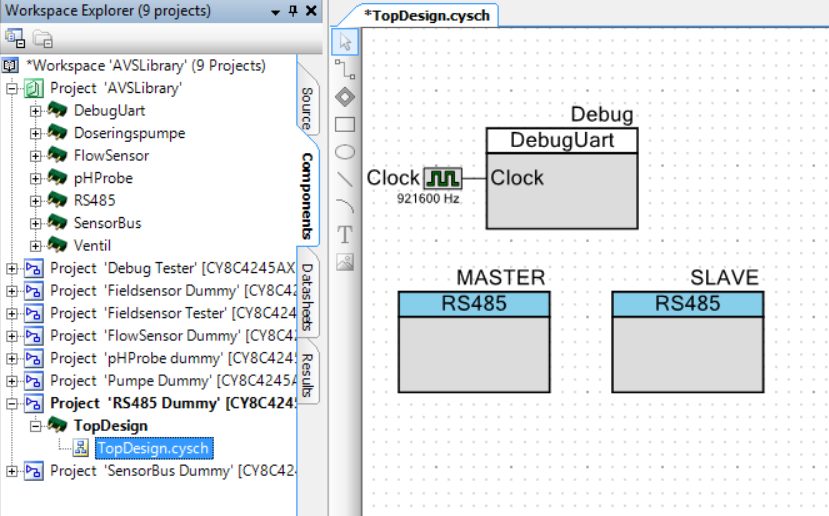
\includegraphics[scale=0.6]{Projektbeskrivelse/DesignOgImplementeringAfSW/AVSLibrary/AVSLibrary.png}
	\caption{AVSLibrary i PSoC creator}
	\label{photo:AVSLibrary}
\end{figure} 

Der er også lavet en række stub projekter til hjælp af udvikling af biblioteket og til at man kan teste interfacing. Dette har gjort det muligt at teste en Fieldsensor uden at have en Sensor Ø klar, og vide at den vil virke med Sensor Ø'en, inden den blev færdigudviklet.

\subsection{RS485}
Da vi havde valgt at bruge RS485 som det fysiske lag for vores bus blev vi også nød til selv at lave en protokol til denne. Det gjorde vi ret simpelt ved at definere hvordan en besked ser ud, det blev til at vi valgte at alle på bussen skulle have en adresse således at vi kunne vælge hvem der skulle skrives til. For at kunne skelne mellem en adresse og en data byte har vi valgt at bruge paritetsbit'en i en UART data frame til at indikere adressen. Vi kører med det der hedder mark/space paritet hvor mark betyder at der står 1 i paritetsbit'en og ved space står der 0, i vores løsning betyder mark paritet at det er en adresse der er sendt og space betyder at det er data. En dybere beskrivelse af kommandoer og dataformat kan læses i systemarkitekturen.